
\documentclass[12pt]{article}
\pagenumbering{gobble}
\usepackage[margin=1.2in]{geometry}

\usepackage[version=4]{mhchem}
\usepackage{float}
\usepackage{tikz}
\usepackage{color, colortbl}
\usepackage{commath}
\usepackage{graphicx}
\usepackage{amsbsy}
\usepackage{hyperref}

\renewcommand*\descriptionlabel[1]{\hspace\leftmargin$#1$}
\newcommand{\ih}{\pmb{\hat{i}}}
\newcommand{\jh}{\pmb{\hat{j}}}
\newcommand{\kh}{\pmb{\hat{k}}}

\graphicspath{ {./} }

\begin{document}

\section{Factors Considered}
The following are factors we calculate and take into account in this design: 
\begin{itemize}
    \item Force exerted on the projectile
    \item Capacitor discharge rate
    \item Heat generated by resistance of rails (Joule heating effect)
    \item Change in resistance as rail temperature increases
\end{itemize}

\section{Simplifying Assumptions}
Following are some factors that are ignored/treated in a simplified manner in this design:
\begin{itemize}
    \item Ignore physical thermal expansion of rails/projectile
    \item Ignore effects of friction on the projectile
    \item Ignore heat transfer between rails, environment, and projectile
    \item Assume resistance of capacitor circuit does not change
    \item Ignore all effects of induction in the rails, projectile, and wiring
    \item Assume no internal resistance/inductance in capacitors
    \item Assume no capacitance in rails and projectile
    \item Assume rails and projectile are infinitely thin when applying Lorentz force law and Biot-Savart law
    \item Ignore magnetic field created by the projectile 
\end{itemize}

\section{Force on the Projectile}

The first step is to calculate the force $F$ exerted on the projectile as a function of the position $x$ of the projectile and the current running through the system (assuming the projectile is within the barrel). We begin by computing the magnitude of the magnetic field generated by one rail (the effective length of the rail is the position of the projectile, as no current flows through the remaining portion of the rail): \\

\begin{center}
    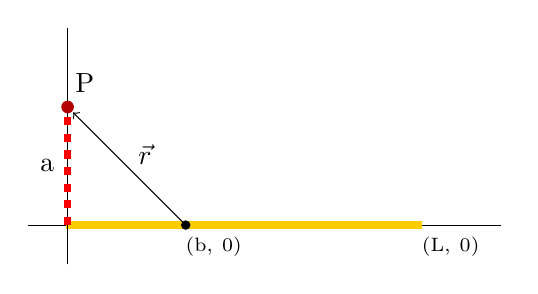
\begin{tikzpicture}
        \draw (0, 0.5) -- (6, 0.5); % node[anchor=south] {x};
        \fill[orange!40!yellow] (0.485, 0.45) rectangle (5, 0.55);
        \draw (0.5, 0) -- (0.5, 3); % node[anchor=east] {y};

        \node[text width=0.2cm] at (0.7, 2.3) {P};
        \draw[red, line width=0.8mm, dashed] (0.5, 0.5) -- (0.5, 2);
        \node[text width=0.2cm] at (0.25, 1.25) {a};
        \fill[red!70!black] (0.5, 2) circle (0.08cm);
        \fill[black] (2.0, 0.5) circle (0.6mm);
        \node[text width=1.0cm] at (2.5, 0.22) {\scriptsize (b, 0)};
        \node[text width=1.0cm] at (5.5, 0.22) {\scriptsize (L, 0)};
        \draw[->] (2.0, 0.5) -- (0.57, 1.93); % node[anchor=east] {y};
        \node[text width=1.0cm] at (1.9, 1.4) {$\vec{r}$};
    \end{tikzpicture}
\end{center}

Given that point $P$ is located at the coordinates $(0, a)$ (as the projectile is always at the end of the portion of the rail which current is running in): 

\begin{equation}
    d\vec{B} = \frac{\mu_0 I d\vec{s} \times \hat{r}}{4\pi \norm{\vec{r}}^2} = 
    \frac{\mu_0 I}{4\pi} \cdot \frac{d\vec{s} \times \hat{r}}{\norm{\vec{r}}^2} = 
    \frac{\mu_0 I}{4\pi} \cdot \frac{d\vec{s} \times \left(\frac{\vec{r}}{\norm{\vec{r}}}\right)}{\norm{\vec{r}}^2} = 
    \frac{\mu_0 I}{4\pi} \cdot \frac{d\vec{s} \times \vec{r}}{\norm{\vec{r}}^3}
\end{equation}
We begin by solving for the infinitesimal portion of the rails:
\begin{equation}
    d\vec{s} = db \ih
\end{equation} 
We then solve for the distance and direction to the point where the magnetic field is being observed:
\begin{equation}
    \vec{r} = (0 - b)\ih + (a - 0)\jh = -b\ih + a\jh
\end{equation}
\begin{equation}
    \norm{\vec{r}} = \sqrt{(-b)^2 + a^2} = \sqrt{b^2 + a^2}
\end{equation}
\begin{equation}
    \norm{\vec{r}}^3 = (b^2 + a^2)^{3/2}
\end{equation}
We then write and simplify the expression for $d\vec{B}$:
\begin{equation}
    d\vec{B} = \frac{\mu_0 I}{4\pi} \cdot \frac{d\vec{s} \times \vec{r}}{\norm{\vec{r}}^3} =
    \frac{\mu_0 I}{4\pi} \cdot \frac{db \ih \times (-b\ih + a\jh)}{(b^2 + a^2)^{3/2}}
\end{equation}
\begin{equation}
    db \ih \times (-b\ih + a\jh) = adb\kh
\end{equation}
\begin{equation}
    d\vec{B} = \frac{\mu_0 I}{4\pi} \cdot \frac{adb\kh}{(x^2 + a^2)^{3/2}}
\end{equation}
We take the norm of $d\vec{B}$ to find the magnitude of the field:
\begin{equation}
    B = \frac{\mu_0 I}{4\pi} \cdot \frac{adb}{(x^2 + a^2)^{3/2}}
\end{equation}
Finally, we integrate along the rail to find $B$ at a given distance $a$ from the rail, where $x$ is the effective length of the rails:
\begin{equation}
    B(a) = \frac{\mu_0 I a}{4\pi} \int_{0}^{x} \frac{db}{(b^2 + a^2)^{3/2}} =
    \frac{\mu_0 I x}{4\pi a \sqrt{x^2 + a^2}}
\end{equation}
Now that we have computed the magnitude of the magnetic field of the rails, we proceed by calculating the force exerted on the projectile. By the right-hand rule, both rails produce a magnetic field such that the force applied on the projectile is forward. Therefore, we can use the Lorentz force law (for a wire) on the projectile (given that $d$ is the separation between the rails and $w$ is the width of the rails): 
\begin{equation}
    F = I \int B ds = I \int_{(w/2)}^{(d + w/2)} B(a) da
\end{equation}
\begin{equation}
    F = I \int_{(w/2)}^{(d - w/2)} \frac{\mu_0 I x}{4\pi a \sqrt{x^2 + a^2}} da = 
    \frac{\mu_0 I^2 x}{4\pi} \int_{(w/2)}^{(d - w/2)} \frac{da}{a \sqrt{x^2 + a^2}}
\end{equation}
Integrating (and doubling, because there are two rails) yields the final expression for force on the projectile when it is a given distance through the barrel (where $x = 0$ is the start of the barrel):
\begin{equation}
    F =
    \frac{2\mu_0 I^2 (\log(d - w/2) - \log(x\sqrt{(d - w/2)^2 + x^2} + x^2) - \log(w/2) + \log(x\sqrt{(w/2)^2 + x^2} + x^2))}{4\pi}
    \label{eqn:eqn1}
\end{equation}

\section{Current in Rails and Projectile}
It follows that the next step is to calculate the amount of current running through the projectile. We first find the resistance of the circuit as a function of time, temperature (which itself is a function of distance along the rails), and effective rail length (position of the projectile).
\begin{equation}
R_{\text{rail}} = \frac{\int\rho\text{ }dl}{A}
\end{equation}
\begin{equation}
\rho(l) = \rho_{0}(1 + \alpha (T(l) - 20)) = \rho_{0}(1 + \alpha T(l) - 20\alpha) = \rho_{0}(1 - 20\alpha) + \rho_{0}\alpha \cdot T(l)
\end{equation}
Given the width of the rail is $w$ and the thickness of the rail is $k$:
\begin{equation}
R_{\text{rail}} = \frac{\int_{0}^{x} \rho(l) dl}{A} = \frac{\rho_{0}(1 - 20\alpha) \int_{0}^{x} dl + \rho_{0}\alpha \int_{0}^{x} T(l) dl}{wk}
\end{equation}
\begin{equation}
R_{\text{rail}} = \frac{\rho_{0}x(1 - 20\alpha) + \rho_{0}\alpha (\int_{0}^{x} T(l) dl)}{wk}
\label{eqn:eqn2}
\end{equation}

We find that the total resistance is (given that $R_{\text{circuit}}$ is the additional resistance of the capacitor circuit and wiring):
\begin{equation}
R_{\text{total}} = 2R_{\text{rail}} + R_{\text{circuit}} = 2\frac{\rho_{0}x(1 - 20\alpha) + \rho_{0}\alpha (\int_{0}^{x} T(l) dl)}{wk} + R_{\text{circuit}} + R_{\text{projectile}}
\label{eqn:eqn3}
\end{equation}

Now, we can use Ohm's law to find the current given a constant voltage source.
\begin{equation}
    V = IR
\end{equation}
\begin{equation}
    I = \frac{V}{R_{\text{total}}}
    \label{eqn:eqn4}
\end{equation}

\section{Temperature Increase of Rails}
By the joule-heating effect, we know that the heat $q$ added to a resistor can be found by the following formula:
\begin{equation}
    q = Pt = I^2 R t 
\end{equation}
Therefore, we can calculate the amount of heat added to a system in a given amount of time:
\begin{equation}
    q = Pt = \left(\frac{Q}{R_{\text{rail}}C}\right)^2 R_{\text{rail}} t = \frac{Q^2 t}{C^2 R_{rail}}
\end{equation}
Next, we need to calculate the change in temperature due to the added heat:
\begin{equation}
    q = mc\Delta T
\end{equation}
\begin{equation}
    \Delta T = \frac{q}{mc}
\end{equation}
The specific heat $c$ will depend on the metal used, and we can calculate the volume and mass as a function of the density $p$ of the metal and the effective length $x$ of the rails:
\begin{equation}
    V = xwk
\end{equation}
\begin{equation}
    m = pV = pxwk
\end{equation}
\begin{equation}
    \Delta T = \frac{q}{pxwkc}
\end{equation}
\begin{equation}
    \Delta T = \frac{\frac{Q^2 t}{C^2 R_{total}}}{pxwkc} = \frac{Q^2 t}{pxwkc \cdot C^2 R_{rail}}
    \label{eqn:eqn6}
\end{equation}
We must note that the increase in temperature only applies between the start of the rail and the point $x$ meters into the rail. Therefore, it must be calculated for every point along the rail.

\end{document}